\newcommand{\todoNK}[1]{\textbf{\textcolor{red}{NK: #1}}}
\chapter{Background}
\label{chapter:background}
\newtheorem{theorem}{Theorem}
In this chapter we present the necessary background that the reader should have in order to proceed through the next two chapters, which are the core of this work. After a brief overview of kernel methods in machine learning, we will present random features and graph kernels. In the next chapter, these different notions will be combined in the proposed algorithm.

\section{Kernel methods and random features}

We first start by an overview of kernel methods.

\subsection{Kernel methods and kernel trick}
Kernel methods is a family of classic algorithms in machine learning that learn models as a combination of similarity functions between data points $(x,x')$, defined by positive semi-definite (psd) \emph{kernels} $\kappa(x,x')$. Denote by $\mathcal{D}$ the set of all possible data points. A symmetric function $\kappa:\mathcal{D}\times\mathcal{D}\mapsto\mathbb{R}$ is said to be a positive semi-definite kernel if:
\begin{equation}
\forall n\in \mathbb{N},~\forall \alpha_1,\ldots,\alpha_n\in \mathbb{R},~\forall x_1,\ldots,x_n\in \mathcal{D},\quad \sum_{i,j}^n\alpha_i\alpha_j\kappa(x_i,x_j)\geq 0 \, .
\end{equation}
Let us now illustrate how kernels can be incorporated to learning models and how that is useful to learn more complex functions. To do that let us consider a classical supervised learning setting for classification: take $\mathcal{D}=\mathbb{R}^d; d\in\mathbb{N}$, and let $\mathcal{X}=(\mathbf{x}_1,\ldots,\mathbf{x}_n)$ be a set of $n$ datapoints in $\mathbb{R}^d$, along with the vector of their associated known labels $\mathbf{y}=(y_1,\ldots,y_n)^T\in\mathbb{R}^n$ where, for each $i$, $y_i$ is the label of the class to which $\mathbf{x}_i$ belongs. For simplicity, we set ourselves in the context of two classes, and we set $y_i=-1$ is $\mathbf{x}_i$ belongs to class $1$, and $y_i=1$ if $\mathbf{x}_i$ belongs to class $2$. 

The classification task is: given this \emph{a priori} known labeled data $(\mathcal{X},\mathbf{y})$, design a classifier that is able to classify any new data point in $\mathbb{R}^d$. 

Many learning models designed to solve this problem, like Support Vector Machine (SVM) \nt{add ref} and Perceptron binary classifier \nt{add ref}, rely on the inner product as a measure of similarity between data points: during the training, they only use inner products $\mathbf{x}_i^T \mathbf{x}_j$, and then produce classifiers with the following form \citep{inner_product}:
\begin{equation}
\label{eq:inner_product}
 \hat{y}(\mathbf{x})=\text{sign}\left\{\sum_{i=1}^n\alpha_iy_i\mathbf{x}_i^T\mathbf{x}\right\} \text{ with } \alpha_i\in \mathbb{R}
\end{equation}
where the values $\{\alpha_i\}_{i=1,\ldots,n}$ in Eq. \ref{eq:inner_product} are optimized based on the dataset $(\mathcal{X},\mathbf{y})$ by the learning algorithm. The intuition behind Eq. \ref{eq:inner_product} is that the output class for every new data point $\mathbf{x}$ is expected to be the same class of nearby points in the input set $\mathcal{D}$. This is achieved by introducing the inner product $\mathbf{x}_i^T\mathbf{x}$ to control how much the class $y_i$ contributes in the output $\hat{y}(\mathbf{x})$. The parameter $\alpha_i$ controls how strongly the data point $x_i$ can affect other neighboring points. They mainly depend on how both classes are distributed in the input set $\mathcal{D}$, and  how much the dataset $(\mathcal{X},\mathbf{y})$ is noisy. 



A \emph{kernel method} consists in replacing every inner products $\mathbf{x}_i^T \mathbf{x}_j$ by a psd kernel $\kappa(\mathbf{x}_i, \mathbf{x}_j)$ during training, and similarly $\mathbf{x}_i^T\mathbf{x}$ by $\kappa(\mathbf{x}_i, \mathbf{x})$ during prediction.
Let us now explain the intuition behind this, starting by rewriting Eq. \ref{eq:inner_product} as 
\[
\hat{y}(\mathbf{x})=\text{sign}\{\textbf{x}^T(\mathbf{X}^T~diag([\alpha]_{i=1}^n)~\mathbf{y})\},
\]
where $\mathbf{X}\in\mathbb{R}^{n\times d}$ is the matrix whose $i$-th row corresponds to data-point $\mathbf{x}_i$, and where $diag([\alpha]_{i=1}^n)$ is the diagonal matrix with values $[\alpha]_{i=1}^n$. 

To get the decision boundary of such classifiers (the boundary in $\mathbb{R}^d$ that separates $\mathbb{R}^d$ into a part associated to class 1 and another associated to class $2$), one solves $\mathbf{x}^T\mathbf{q}=\mathbf{0}$, where $\textbf{q}=(\mathbf{X}^T~diag([\alpha]_{i=1}^n)~\mathbf{Y})\in\mathbb{R}^d$. It is the equation of a hyper-plane in the input space $\mathbb{R}^d$, also referred to as a \emph{linear} decision boundary. 
The question here is: what if the two classes are not separable by a hyper-plane (as illustrated on the left of Fig. \ref{fig:SVM_boundaries})? 

\begin{figure}[t]
	\centering
	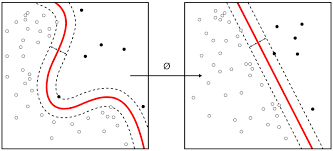
\includegraphics[scale=0.5]{figs/svm.png}
	\caption[The case where classes aren't separable using linear boundary]{The left figure shows a case where the input data in their original space are not separable by a linear boundary. The right figure shows the same data transformed to a new space using a lifting function $\varphi$, and we can see that different classes are now separable  using linear boundary. \nt{in fact, I would remove $\varphi$ from this figure and only use this figure to show an example on the right of a linearly separable dataset; and an example on the left where it is not the case. Justifying the use of a mapping $\varphi$ is the message of Fig.~\ref{fig:polynomial_kernel}}}
	%Source:
	\label{fig:SVM_boundaries}
\end{figure}

One common solution to this problem is to map the data points from $\mathbb{R}^d$ to another space $\mathbb{R}^m$  through a proper mapping function $\varphi$ such that the two classes become separable with a linear decision boundary in $\mathbb{R}^m$. Then we can apply the same learning models specified in Eq. \ref{eq:inner_product} but on the transformed data. Let us consider for example the dataset shown in Fig. \ref{fig:polynomial_kernel},  we can use the following mapping function $\varphi:(x_1,x_2)\mapsto (\sqrt{2}x_1x_2,x_1^2,x_2^2)$ to move from $\mathbb{R}^2$ on the left, where data are not linearly separable, to $\mathbb{R}^3$ on the right, where they are.

\begin{figure}[t]
\centering
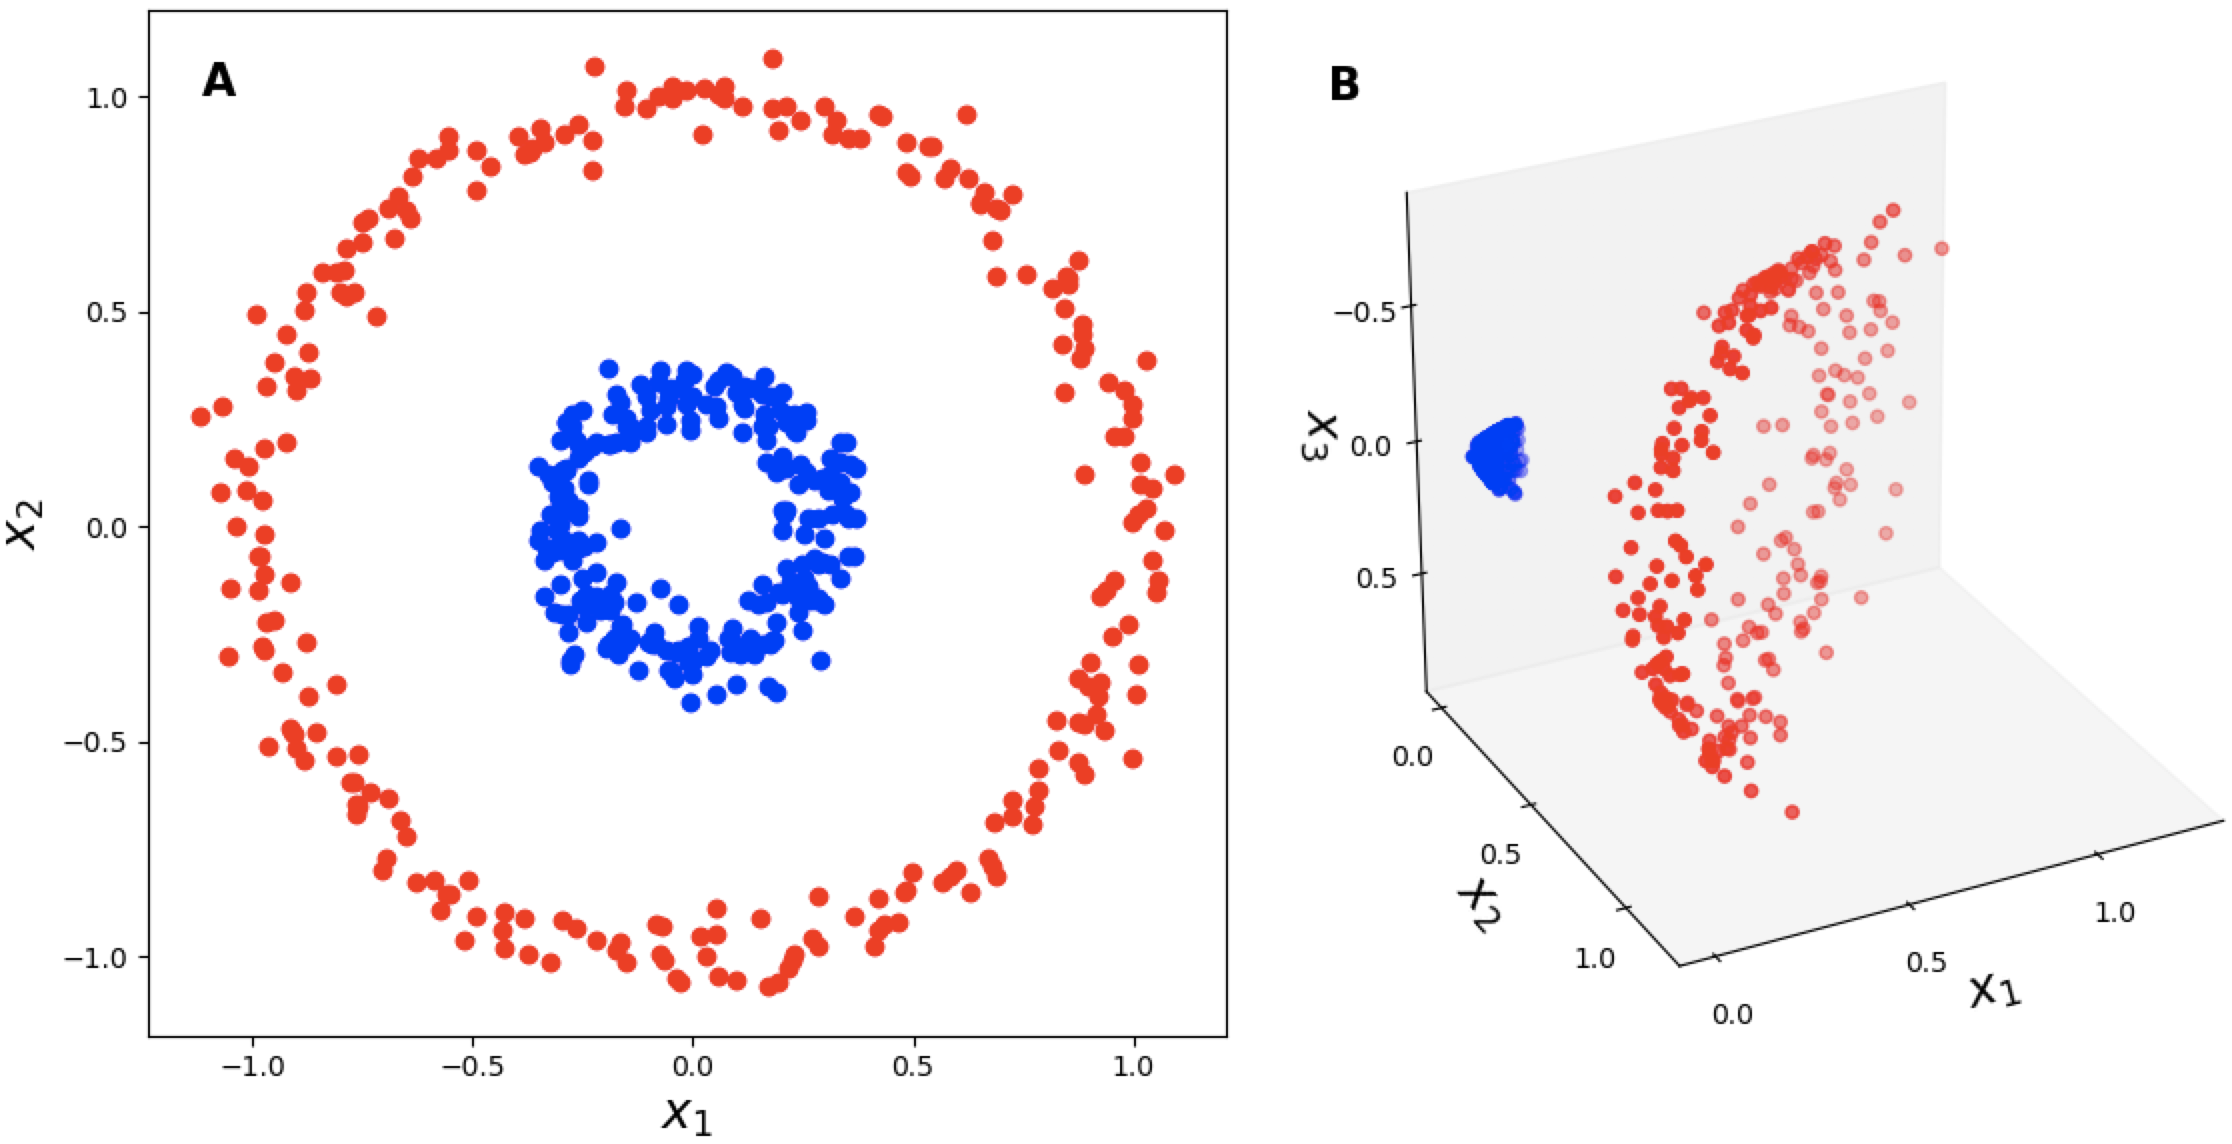
\includegraphics[scale=0.25]{figs/poly_kenrnel.png}
\caption[Lifting data to a higher-dimension space to get linearly separable classes]{ Using the mapping function $\varphi:(x_1,x_2)\mapsto (\sqrt{2}x_1x_2,x_1^2,x_2^2)$ to map the data on the left in $\mathbb{R}^2$ to $\mathbb{R}^3$ where they are linearly separable}
%Source:
\label{fig:polynomial_kernel}
\end{figure}

Learning such a function $\varphi$ is what is typically done by neural networks using complex optimization methods.  Kernel methods are much simpler (and elegant) methods to perform this mapping. They are justified by the following key theorem.

\begin{theorem}[Mercer theorem]
To every positive semi-definite kernel $\kappa:\mathbb{R}^d\times \mathbb{R}^d\mapsto \mathbb{R}$, there exists a Hilbert space $\mathbb{H}$ and a feature map $\phi:\mathbb{R}^d\mapsto\mathbb{H}$ such that for all $\mathbf{x},\mathbf{x}'\in\mathbb{R}^d$ one has:: 
\begin{equation}
\label{eq:kernel_main_equation}
    \kappa(\mathbf{x},\mathbf{x}')=<\phi(\mathbf{x}),\phi(\mathbf{x}')>_\mathbb{H}
\end{equation}
where $<\phi(\mathbf{x}),\phi(\mathbf{x}')>_\mathbb{H}$ is the inner product defined in $\mathbb{H}$.
\end{theorem}

This theorem states that replacing the inner product $\mathbf{x}_i^T\mathbf{x}$ in Eq. \ref{eq:inner_product} by a positive semi-definite kernel $\kappa(\mathbf{x}_i,\mathbf{x})$ is equivalent to implicitly map the data from the original input space $\mathcal{D}$ to another feature space $\mathbb{H}$ and then apply the classical inner product. Therefore, one \emph{does not need to know explicitely the mapping} $\phi$ nor the new feature space $\mathbb{H}$, instead, it is sufficient to evaluate the kernel $\kappa$ for pairs of data points in the original input space $\mathcal{D}$. This main feature of kernel methods is known as the \emph{kernel trick}. It has two main advantages:
\begin{itemize}
    \item Kernels allow us to transform data to a new Hilbert space of very high or even infinite dimensionality, which can make the learning model able to represent more complex functions.
    \item Kernels are often computationally cheaper, since they save the time required to compute the explicit co-ordinates of the data in the new feature space by directly calculating the inner product between the transformed data.
\end{itemize}
To better illustrate these benefits, we take the Gaussian kernel as an example, which is one of the most classical kernels in $\mathbb{R}^d$, defined as:
\begin{equation}
\label{eq:Guassian_kernel}
    \kappa_{G}(\mathbf{x},\mathbf{x}')=\exp^{-\frac{\left \| \mathbf{x}-\mathbf{x}'\right\|^2}{2\sigma^2}}
\end{equation}
where $\sigma>0$ is the bandwidth parameter of the kernel. The lifting function $\phi_G$ of this kernel is located in a Hilbert space of infinite dimension \nt{add ref}, but the kernel can be easily evaluated for any pair $(\mathbf{x},\mathbf{x}')\in\mathbb{R}^d\times \mathbb{R}^d$.

Despite their advantages, kernel methods still have some drawbacks, notably in the computation of the Gram matrix. The Gram matrix associated to a given kernel $\kappa$ and a given set $\mathcal{X}$ of $n$ datapoints in $\mathbb{R}^d$, is a matrix of size $n\times n$ whose $(i,j)_{th}$ entry equals the kernel evaluated between points $\mathbf{x}_i$ and $\mathbf{x}_j$: $\kappa(\mathbf{x}_i, \mathbf{x}_j)$. This Gram matrix is typically needed to learn the parameters $\{\alpha_i\}$ of the classifier. Computing this matrix takes however $\mathcal{O}(dn^2)$ operations and requires $\mathcal{O}(n^2)$ memory space. As $n$ and/or $d$ increase, these computation and memory costs may become prohibitive. 
\nt{** this last paragraph needs some work still. The memory argument is not really an argument. In fact, the GRam matrix, whatever the dimension of the embedding, always needs $\mathcal{O}(n^2)$ to be stored. What RFF truly provide is a low rank approximation of the Gram matrix.}

%\begin{itemize}
 %   \item The Gram matrix associated to a given kernel $\kappa$ and a given set $\mathcal{X}$ of $n$ datapoints in $\mathbb{R}^d$, is a matrix of size $n\times n$ whose $(i,j)_{th}$ entry equals the kernel evaluated between points $\mathbf{x}_i$ and $\mathbf{x}_j$: $\kappa(\mathbf{x_i}, \mathbf{x_j})$. This Gram matrix is typically needed to learn the parameters $\{\alpha_i\}$ of the classifier. Computing this matrix takes however $\mathcal{O}(dn^2)$ operations and requires $\mathcal{O}(n^2)$ memory space. As $n$ and/or $d$ increase, these computation time and memory costs may become prohibitive. 
 %   Since for most kernels we need to evaluate the kernel on each pairs of data points, for a dataset $(\mathbf{X},\mathbf{X})$ \nt{?} of size $n$, we need $O(n^2)$ memory entries to compute what is called a Gram matrix, .
 %   \item Even if most kernels are designed so that they can be evaluated in polynomial time in the dimensionality of the input space $\mathcal{D}$ (for instance computing $\mathcal{K}_{G}(\mathbf{x},\mathbf{x}')$ for two vectors in $\mathbb{R}^d$ costs $d$ operations),  some kernels (especially on graphs) are computationally expensive \citep{graphlet_kernel}. \todoNK{I would not mention that here, since handling exponential computation of *each individual evaluation* of the kernel with RF is precisely what we do which has not been done before. Only the Gram matrix problem is mentioned in the original RF paper.}
%\end{itemize}

To overcome these difficulties, random feature projections is a technique developed to approximate kernels, often requiring less computational time and less memory storage.

\subsection{Random features}
Random features (RF) \citep{rahimi2008random} is an approach developed to approximate kernel methods with reduced computational time. The idea is that, instead of considering the true lifting function $\phi$ in Eq. \ref{eq:kernel_main_equation}, we explicitly map the data points using an appropriate randomized feature map $\varphi:\mathcal{D} \xrightarrow{}\mathbb{C}^m$, such that the kernel evaluated for two data points $\mathbf{x}, \mathbf{x}'$ is approximated by the inner product of their random features with high probability:
\begin{equation}
\label{eq:approx_RF}
\kappa(\mathbf{x},\mathbf{x}')=<\phi(\mathbf{x}),\phi(\mathbf{x}')>_\mathbb{H} \approx \varphi(\mathbf{x})^*\varphi(\mathbf{x}')
\end{equation}
where $^*$ stands for the conjugate transpose. 
Considering this approximation, we can transform the input vectors of $\mathcal{X}$ with $\varphi$ and then apply a linear learning method as in Eq. \ref{eq:inner_product} to have a similar learning power as the original non-linear kernel machine, while often avoiding the cost of explicitly constructing the Gram matrix. Note that with RF we do not use the kernel trick anymore, but construct an explicit (even if random) mapping $\varphi$ to approximate the kernel $\kappa$.

Most RF constructions are known as Random \emph{Fourier} Features (RFF), and are based on the following theorem.
\begin{theorem}[Bochner's theorem]
A continuous and shift-invariant kernel $\kappa(\mathbf{x},\mathbf{x}')=\kappa(\mathbf{x}-\mathbf{x}')$ on $\mathbb{R}^d$ is positive definite if and only if $\kappa$ is the Fourier transform of a non-negative measure.
\end{theorem}
As a direct consequence, we can easily scale any shift-invariant kernel to obtain $\kappa(0) = \int p = 1$, so that its Fourier transform $p(\mathbf{w})$ is a correct probability distribution. We obtain that any shift-invariant psd kernel is of the form:
\begin{equation}
\label{Fourier integral}
\kappa(\mathbf{x}-\mathbf{x}')=\int_{\mathbb{R}^d}p(\mathbf{w})e^{j\mathbf{w}^T(\mathbf{x}-\mathbf{x}')}d\mathbf{w}= E_{\mathbf{w}\sim p}[\xi_\mathbf{w}(\mathbf{x})^*\xi_\mathbf{w}(\mathbf{x}')]
\end{equation}
where $\xi_\mathbf{w}(\mathbf{x})=e^{-j\mathbf{w}^T\mathbf{x}}$ and where $E_{\mathbf{w}\sim p}$ stands for the expectation over $\mathbf{w}$ drawn from the probability distribution $p(\mathbf{w})$. Note that, since $\kappa$ is a real-valued function, from Eq.~\ref{Fourier integral} one can also prove that:
\begin{equation}
\label{real Fourier integral}
\kappa(\mathbf{x}-\mathbf{x}')=\int_{\mathbb{R}^d}p(\mathbf{w})cos({\mathbf{w}^T(\mathbf{x}-\mathbf{x}')})d\mathbf{w}=E_{\mathbf{w}\sim p}[\tilde \xi_\mathbf{w}(\mathbf{x})\tilde \xi_\mathbf{w}(\mathbf{x}')]
\end{equation}
where $\tilde \xi_\mathbf{w}(\mathbf{x})=\sqrt{2}cos(\mathbf{w}^T\mathbf{x}+b)$ such that $\mathbf{w}$ is drawn from $p$ and $b$ is drawn uniformly from $[0,2\pi]$, such that we can use a real-valued mapping if desired.

As a result, for $\mathbf{w}$ a random variable drawn from $p(\mathbf{w})$, $\  \xi_\mathbf{w}(\mathbf{x})^*  \xi_\mathbf{w}(\mathbf{x}')$ is an unbiased estimate of $\kappa(\mathbf{x},\mathbf{x}')$. The RF methodology consists in averaging $m$ instances of the estimator with different random frequencies $\mathbf{w}_j$ drawn identically and independently (iid) from $p$, that is, define
\begin{align}
\label{eq:Fourier_xi}
\varphi(\mathbf{x}) = \frac{1}{\sqrt{m}} ( \xi_{\mathbf{w}_j}(\mathbf{x}) )_{j=1}^m \in \mathbb{C}^m
\end{align}
such that $\varphi(\mathbf{x})^*\varphi(\mathbf{x}')=\frac{1}{m} \sum_{j=1}^m \xi_{\mathbf{w}_j}(\mathbf{x})^*\xi_{\mathbf{w}_j}(\mathbf{x}')$, which converges to $\kappa(\mathbf{x},\mathbf{x}')$ by the law of large numbers. Moreover, Hoeffding's inequality guarantees exponentially fast convergence in $m$ between $\varphi(\mathbf{x})^*\varphi(\mathbf{x}')$ and the kernel's true value:
\begin{equation}
   \forall \epsilon >0\qquad Pr(|\varphi(\mathbf{x})^*\varphi(\mathbf{x}')-\kappa(\mathbf{x},\mathbf{x}')|\geq\epsilon)\leq2e^\frac{-m\epsilon^2}{4},
\end{equation}
that is, for any error $\epsilon>0$, the probability that the estimation is off by more than $\epsilon$ is controlled by an exponentially decaying term.

One could use the union bound on all couples $(\mathbf{x},\mathbf{x}')\in\mathcal{X}^2$ to study the  concentration of \emph{all} entries of the Gram matrix, not only a given couple as in the previous Hoeffding inequality:
\begin{theorem}[\nt{add ref}]\label{thm:RF_vs_logn}
Let $\epsilon\in(0,1)$ and $\delta\in(0,1)$. Consider a dataset $\mathcal{X}=(\mathbf{x}_1,\ldots,\mathbf{x}_n)$ of $n$ elements, and a psd shift-invariant kernel $\kappa$. The random embedding  $\varphi(\mathbf{x})\in\mathbb{C}^m$ defined in Eq.~\eqref{eq:def_RF} enables a controlled approximation of \emph{all} the elements of the Gram matrix with probability larger than $1-\delta$, \emph{i.e.}
$$\text{Pr}\left(\forall (\mathbf{x}, \mathbf{x}')\in\mathcal{X}^2\quad|\varphi(\mathbf{x})^*\varphi(\mathbf{x}')-\kappa(\mathbf{x},\mathbf{x}')|\leq\epsilon\right)\geq 1-\delta$$ 
provided that 
$$m\geq\mathcal{O}\left(\frac{1}{\epsilon^2}\log{\frac{n}{\delta}}\right).$$
\end{theorem}

As an illustration, consider the Gaussian kernel in Eq. \ref{eq:Guassian_kernel}. This kernel is shift-invariant and known to be positive semi-definite. It is already correctly normalized since $\kappa(0) = 1$, and its Fourier transform is also a Gaussian but with inverted variance:
\begin{equation}
\label{eq:G_fourier}
p(w)=FT\big(\kappa_G\big)(\mathbf{w})=\left(\frac{\sigma^2}{2\pi}\right)^\frac{d}{2}e^{-\frac{\sigma^2\|\mathbf{w}\|^2}{2}}
\end{equation}
Thus, in practice, in order to approximate the Gram matrix of $\kappa_G$ on a dataset $\mathcal{X}$ of size $n$, one i/~draws $m$ iid frequencies from this probability distribution, with $m$ as in Theorem~\ref{thm:RF_vs_logn}; ii/~uses these frequencies to associate to each element $\mathbf{x}\in\mathcal{X}$ its associated random feature vector $\varphi(\mathbf{x})\in\mathbb{C}^m$ as defined in Eq.~\eqref{eq:def_RF}  (or its real-valued equivalent in $\mathbb{R}^m$); iii/~uses $\varphi(\mathbf{x})^*\varphi(\mathbf{x}')$ as an approximation of $\kappa_G(\mathbf{x},\mathbf{x}')$ where necessary in any kernel-based learning algorithms.

\section{Graphlet kernel}
Kernel methods are a flexible set of tools, since psd kernels can be defined on any set of objects rather than on vectors $\mathbf{x}\in \R^d, d\in \mathbb{N}$. Naturally, for machine learning tasks on graphs such as graph classification or regression, authors have developed kernels on graphs $\kappa(\mathcal{G},\mathcal{G}')$~\citep{kriege_graph_kernels}. This section gives a brief overview of graph kernels, focusing on the so-called \emph{graphlet kernel}, which will be our main inspiration for this work. 
\nt{Present the table of contents: section 221 will... In section 222 the.. will be detailed before we present, in section 223, ...}

\subsection{Notations of graphs and graphlets}
Recall that a graph $\mathcal{G} = (\mathcal{V}, \mathcal{E})$ is formed by a set of nodes and a set of edges connecting them. A graph $\mathcal{F}=(\mathcal{V}_\mathcal{F},\mathcal{E}_\mathcal{F})$ is said to be a subgraph (also called \emph{graphlet}) of $\mathcal{G}$, written $\mathcal{F}\sqsubseteq \mathcal{G}$, if and only if there exists an injective function $g:\mathcal{V}_\mathcal{F}\xrightarrow{} \mathcal{V}$ such that $(u,u')\in \mathcal{E}_\mathcal{F} \Leftrightarrow{(g(u),g(u'))\in \mathcal{E}}$.

Any edge $(u_i, u_i)$ is called a self loop. In a general graph two vertices $u_i$ and $u_j$ may be connected by more than
one edge. A simple graph is a graph with no self loops or multiple edges. Here we always consider simple graphs.
A (simple) graph can equivalently be represented by an adjacency matrix $\mathbf{A}$ of size $v \times v$. The $(i,j)-th$ entry of $\mathbf{A}$ is 1 if an edge $(u_i, u_j)$ exists and zero otherwise.

Two graphs $\mathcal{G}=(\mathcal{V},\mathcal{E})$ and $\mathcal{G'}=(\mathcal{V'},\mathcal{E'})$ are said to be \emph{isomorphic}, written $\mathcal{G}'\cong \mathcal{G}$, if there exists a bijective function $g:\mathcal{V}\xrightarrow{} \mathcal{V}'$ such that $(u_i,u_j)\in \mathcal{E}$ iff $(g(u_i),g(u_j))\in \mathcal{E}'$. Deciding if two graphs are isomorphic is known to be a difficult problem: it is actually an open question if this problem is solvable in polynomial time or is NP-complete \nt{add ref}. It is equivalent to test if two adjacency matrices are a permutation of each other. This gives us a clue why the isomorphism test is expensive: in the worst case where the graphs to be compared don't have a specific structure which can used as \emph{a prior}, the brute force method considers all the $v!$ permutation matrices. There are efficient, specific methods for small graphs \citep{graphlet_kernel}, but the general case is still open \nt{add ref}. We denote by $C^{\cong}_k$ the computational cost of testing the isomorphism between two graphs of size $k$. 

As we will see, for a given graph, the graphlet kernel is defined by counting small subgraphs of size $k$, also called graphlets. We here introduce some useful notations. Let us denote by $\mathfrak{H}=\{\mathcal{H}_1,..., \mathcal{H}_{N_k}\}$ the set of all possible graphlets of size $k$. Depending on the context, there is two choices in defining this set. Either we count all possible adjacency matrices and treat isomorphic graphs as different graphs, in which case we have $N_k=2^{k(k-1)/2}$ different graphlets. We refer to this set as the set of graphlets \emph{with repetition}. Or we do not distinguish isomorphic graphs, in which case $N_k<2^{k(k-1)/2}$ but it is still exponential in $k$. We call this set the set of graphlets \emph{without repetition}. The classical graphlet kernel uses graphlets without repetition, which can require expensive isomorphism tests. We will see that some methods on graphlets \emph{with} repetition also perform well in practice.

Say we sample a graphlet $\mathcal{F}$ of size $k$ from a given graph $\mathcal{G}$. A possibly expensive operation is to find, in the set $\mathfrak{H}$ of all possible graphlets of size $k$, which one it matches. We define the matching function $\varphi_{k}^{match}$ which, in the case of graphlets with repetition is defined as: 
\[
\varphi_k^{match}(\mathcal{F}) = \left[ 1_{(\mathcal{F} = \phlet_i)}\right]_{i=1}^{N_k}= \left[ 1_{(\mathbf{A}_\mathcal{F} = \mathbf{A}_{\phlet_i})}\right]_{i=1}^{N_k} \in \{0,1\}^{N_k}
\]
where $1_{(\Omega)}$ is the indicator function: it equals $1$ if the proposition $\Omega$ is true, and $0$ otherwise. 
In words, $\varphi_k^{match}(\mathcal{F})$ is a Boolean vector of dimension $N_k$ and has a $1$ in the coordinate $i$ if the adjacency matrices of both graphs $\mathcal{F}$ and $\phlet_i$ are equal, and $0$ otherwise. Clearly the cost of each test is $k^2$, and the cost of applying $\varphi^{match}_k$ to any graph $\mathcal{F}$ is\footnote{\nt{This is in fact the cost of a naive implementation. First of all, as soon as a match is found, one does not need to check for other possibilities and may stop the algorithm. Also, ordering all possible adjacency matrices according to a smart tree-search algorithm would certainly decrease this cost. We will not delve into this here.}} $\mathcal{O}(N_k k^2)$. 

In the case of graphlets \emph{without repetition}, $\varphi_k^{match}$ is defined as:
\[
\varphi_k^{match}(\mathcal{F}) = \left[ 1_{(\mathcal{F} \cong \phlet_i)}\right]_{i=1}^{N_k} \in \{0,1\}^{N_k}
\]
which means that $\varphi_k^{match}$ puts a $1$ in the coordinate $i$ if $F\cong \phlet_i$, and $0$ otherwise. The cost global cost of applying $\varphi^{match}_k$ to any graph $\mathcal{F}$ is now $\mathcal{O}(N_k C^{\cong}_k)$, with an isomorphic test cost $C^{\cong}_k$ exponential in $k$ thus much larger than $k^2$, although for a $N_k$ smaller than the case with repetition.  

Let $\mathfrak{F}$ be any collection of size-$k$ graphs. We define the function $\varphi_k^{hist}$ which counts, for each graphlet $\phlet_i$ in $\mathfrak{H}$, how many matches it has in $\mathfrak{F}$. This definition exists for both versions of $\varphi_k^{match}$, and reads:
\begin{align}
	\label{eq:def:phi_hist}
\varphi_k^{hist}(\mathfrak{F})=\frac{1}{s}\sum_{\mathcal{F}\in\mathfrak{F}} \varphi_k^{match} (\mathcal{F}) \in \R^{N_k}
\end{align}
where the term $\frac{1}{s}$ is introduced for normalization purposes: in order for  $\varphi_k^{hist}(\mathfrak{F})$ to sum to 1. %With this definition and when $s$ is sufficiently large, $\varphi_k^{hist}(\mathbf{F}_\G)$ can be seen as the vector whose $i_{th}$ entry has the frequency of graphlet $\phlet_i$ in the graph $\G$.


\subsection{Convolutional graph kernels}
\nt{**I only partially corrected the notations in this section**}
Recall that traditional kernel machines are applied to problems with vector-valued input data, where they compare different data points $\mathbf{x},\mathbf{x}' \in \mathbb{R}^d$, often through their Euclidean distance. Based on that, these kernels cannot be used directly on (a vector representation of the) graphs: indeed, isomorphic graphs have different adjacency matrices representing the same structure. As a result it is necessary to measure distances between graphs in ways that are insensitive to isomorphism: ideally, if $\mathcal{G}_1 \cong \mathcal{G}'_1$ and $\mathcal{G}_2 \cong \mathcal{G}'_2$, then $\kappa(\mathcal{G}_1, \mathcal{G}_2)$ should be equal to, or at least very close to, $\kappa(\mathcal{G}_1', \mathcal{G}_2')$. One observes that the concept of isomorphism is critical in learning algorithms on graphs, not only because there is no known polynomial-time algorithm for testing graph isomorphism (except for graphs with specific structures), but simply testing isomorphism is also too strict for learning in a similar way to learning with equality operator \nt{not able to re-write this last sentence: I do not understand it} \citep{kriege_graph_kernels}.

Since it is simpler to define kernels on \emph{small} graphs, most of the graph kernels in the literature belong to the family of \emph{convolution kernels}: given two graphs, the trick is to divide each into smaller subgraphs and then to pairwise compute a kernel between the resulted subgraphs.
\newtheorem{definition}{Definition} 
\begin{definition}[Convolution Kernel]
let $\mathcal{R}=\mathcal{R}_1\times...\times \mathcal{R}_d$ denote a space of components such that a composite object $X\in \mathcal{X}$ decomposes into elements of $\mathcal{R}$. Let $R:\mathcal{R}\xrightarrow{}\mathcal{X}$ denote the mapping from components to objects, such that $R(x)=X$ iff the components $x\in \mathcal{R}$ make up the object $X\in \mathcal{X}$, and let $R^{-1}(X)=\{x\in\mathcal{R}:R(x)=X\}$. then, the R-convolution kernel is:
\begin{equation}
\label{eq:conolutional_kernels}
    K_{CV}(X,Y)=\sum_{x\in R^{-1}(X)}~\sum_{y\in R^{-1}(Y)}~\underbrace{\prod_{i=1}^{d}k_i(x_i,y_i)}_{k(x,y)}
\end{equation}
with $k_i$ is a kernel on $\mathcal{R}$ for $i\in\{1,...,d\}$.
\end{definition}

Applying this definition on graphs, $R^{-1}(\mathcal{G}=(\mathcal{V},\mathcal{E}))$ includes all the components in graph $\mathcal{G}$  that we want to compare with the components $R^{-1}(\mathcal{G'}=(\mathcal{V}',\mathcal{E}'))$ in graph $\mathcal{G'}$. One example of these kernels is the node label kernel, where for two graphs $\mathcal{G}, \mathcal{G'}$, the mapping function $R$ maps the features $x_u\in \mathcal{R}$ of each node $u\in \mathcal{V}\cup \mathcal{V'}$ to the graph that $u$ is a member of. Another example, which will be our main source of inspiration and will be further described in the next section, is the $k$-graphlet kernel, where $R$ here maps the subgraphs of size $k$ to the graph in which they occur.
 
The advantage of using convolution kernel framework with graphs is that kernels are permutation invariant, non-sensitive to  on the graphs level as long as they are permutation invariant on the components level. As a drawback, the sum in Eq.~\ref{eq:conolutional_kernels} iterates over every possible pair of components. As a result, when the base kernel has high value between a component and itself while it is low between two different components, each graph becomes drastically similar to itself but distant from any other graph. Thus, a set of weights is usually added to counter-balance this problem.

\subsection{Graphlet Kernel}
\label{subsection: graphlet kernel}

As mentioned above, the graphlet kernel is a special instance of convolution kernel equivalently described as follows: one enumerates all the subgraphs of size $k$ of each graph (where $k$ is small), counts them to build a histogram of their frequencies of apparition, and takes the inner product between the two histograms to obtain the final kernel. In this context, the subgraphs are called ``graphlets'', as an analogy with classical wavelets, which are individual components of more traditional signals.


For a graph $\mathcal{G}=(\V,\E)$, denote by $\mathfrak{F}_\G=\{\mathcal{F}_1,\mathcal{F}_2,\ldots,\}$ the exhaustive collection of \emph{all} size-$k$ subgraphs existing in $\G$: $\mathfrak{F}_\G$ thus has $\tbinom{v}{k}$ elements. Let us define the $k$-spectrum of $\G$: the vector $\mathbf{f}_\G$ of size $N_k$ obtained when applying the function $\varphi_k^{hist}$ as defined in Eq.~\eqref{eq:def:phi_hist} to  $\mathfrak{F}_\G$:
\[
\mathbf{f}_\G=\varphi_k^{hist}(\mathfrak{F}_\G) \in\mathbb{R}^{N_k}
\]
In words, the $i$-th of $\mathbf{f}_\G$ equals the frequency of appearance of graphlet $\mathcal{H}_i$ in $\mathcal{G}$. Classically, the graphlets are considered without repetition. We will sometimes refer to $\mathbf{f}_\G$ simply as the histogram of $\G$. 

The graphlet kernel between two graphs is the inner product between their histograms:
\begin{definition}[Graphlet Kernel]
Given two graphs $\mathcal{G}$ and $\mathcal{G}'$ of size $\geq k$, the graphlet kernel $\mathcal{K}_\G$ is defined as \citep{graphlet_kernel}:
\begin{equation}
\label{eq:graphlet_kernel}
    \mathcal{K}_g(\mathcal{G},\mathcal{G}')=f_{\mathcal{G}}^Tf_{\mathcal{G}'}.
\end{equation}
\end{definition}
In this case the distance between graphs in the kernel space is just the Euclidean metric between histograms $d_\kappa({\mathcal{G}},{\mathcal{G}'}) = \|\mathbf{f}_{\mathcal{G}} - \mathbf{f}_{{\mathcal{G}'}}\|_2$. Also, from now on, unless otherwise specified, $\kappa$ will refer to this graphlet kernel. 

The computational cost is a major drawback of this kernel, as computing the $k$-spectrum vector $\mathbf{f}_{\mathcal{G}}$ of any graph $\G$ is very costly, even for moderate $k$: the sum of Eq.~\eqref{eq:def:phi_hist} is over $\mathfrak{F}_\G$, thus over $\tbinom{v}{k}$ elements; and since graphlets are taken without repetition isomorphism tests have to be performed. Thus, the total cost for computing $\mathbf{f}_{\mathcal{G}}$ can be written as:
\begin{equation}
\label{eq:cost_graphlet}
    C_{gk}= \mathcal{O}(\tbinom{v}{k} N_k C^{\cong}_k).
\end{equation}
As a result, there is a trade-off between a more accurate representation of the graph (larger value of $k$) and the computational cost. However, one can take advantage of some techniques in order to handle this limitation. In the next section, we focus on random sampling.


\subsection{Graph sampling to approximate the $k$-graphlet spectrum}
\label{graph_sampling}
%Graph sampling arises when we deal with a large-scale graph and the task is to pick a small-size sample subgraph that would be similar to the original graph with respect to some important properties.

The graphlet kernel can be interpreted as follows: if one draws a subgraph uniformly at random from $\mathcal{G}$, then one has a probability $(\mathbf{f}_\mathcal{G})_i$ of obtaining $\mathcal{H}_i$, \emph{i.e.}:
$$\mathbf{f}_\mathcal{G} = \mathbb{E}_{F \sim {\rm unif}} ~\varphi^{match}_k(F)$$
where $\mathbb{E}_{F \sim {\rm unif}}$ stands for the expectation over the subgraphs $F$ of size $k$ drawn uniformly at random. Note that we use the notation $F$, instead of $\mathcal{F}$, when the subgraph it refers to is a random variable. 

It is thus natural to approach $\mathbf{f}_\mathcal{G}$ with a sample average, built by i/~first uniformly sampling at random $s$ subgraphs of size $k$ from $\G$ to form the collection 
$$\hat{\mathfrak{F}}^{\rm u}_\G=\{F_1,...,F_s\}$$
and ii/~then estimate the $k$-spectrum vector from these random samples:
\begin{align}
	\label{eq:fhat_unif}
	\hat{\mathbf{f}}_\mathcal{G}^{\rm u} = \varphi_k^{hist}(\hat{\mathfrak{F}}^{\rm u}_\G)= \frac{1}{s}\sum_{F\in\hat{\mathfrak{F}}^{\rm u}_\G} \varphi^{match}_k(F).
\end{align}
In words, the $i$-th entry of $\hat{\mathbf{f}}^{\rm u}_\mathcal{G}$ counts the number of times $\mathcal{H}_i$ appears among the samples. 
The law of large numbers states that $\hat{\mathbf{f}}^{\rm u}_\G \xrightarrow[s \to \infty]{} \mathbf{f}_\mathcal{G}$ with probability $1$.
The question here is how many samples we should consider in order to have a desired certainty in our estimation. In other words: how fast is the concentration of $\hat{\mathbf{f}}^{\rm u}_\G$ around $\mathbf{f}_\G$? The following theorem answers this question:% for every sampling technique $S_k$ whose corresponding $\varphi_k^{hist}$ converge to $f_\G$ when the number of sample grows to infinity.
%\newtheorem{theorem}{Theorem} 
\begin{theorem}[\citep{graphlet_kernel}]
	\label{thm:norm1}
	Let $\mathbf{f}_\G$ be the $k$-spectrum of a graph $\mathcal{G}$. Let $\hat{\mathfrak{F}}^{\rm u}_\G=\{F_1,...,F_{s}\}$ be a collection of $s$ iid random subgraphs of size $k$ uniformly drawn from $\mathcal{G}$ and $\hat{\mathbf{f}}^{\rm u}_G$ the associated estimation of $\mathbf{f}_G$ as defined in Eq.~\eqref{eq:fhat_unif}. Then, for a given $\epsilon>0$ and $\delta >0$, one only needs:
	\begin{equation}
	s_{min}=\left \lceil \frac{2(N_k\log(2)+\log(\frac{1}{\delta} ))}{\epsilon^2} \right \rceil
	\end{equation}
	samples to ensure that $Pr(\| \mathbf{f}_\G-\hat{\mathbf{f}}^{\rm u}_G \|_1 \geq \epsilon )\leq\delta$, where $\lceil.\rceil$ is the ceiling function.
\end{theorem}
\nt{add comment?}

\noindent\textbf{Other random sampling techniques.} In fact, many other random sampling techniques can be used to sample subgraphs from all the possible ones \citep{graph_sampling}: uniform sampling is only one such possibility. A \emph{sampling method} will generically be denoted by $S_k$. We will denote by $F \sim S_k(\G)$ a random subgraph of size $k$ of $\G$ sampled by $S_k$. Note that each sampling method defines a potentially \emph{different histogram}\footnote{We use generically the notation $\mathbf{f}_\G$ for histograms. The underlying sampling method should be clear from context.} $\mathbf{f}_\G = \mathbb{E}_{F \sim S_k(\G)} \varphi^{match}_k(F)$, that can in turn be estimated with a sample average as in the previous uniform case. These different histograms capture different kinds of information from the graph $\G$ and may all potentially be used to solve graph learning problems. We describe two examples that we will use in the experiments.
\begin{itemize}
\item \textbf{Uniform sampling} is the simplest sampling method. We select a subset of $k$ nodes uniformly at random among the $\tbinom{v}{k}$ possible choices, and extract the subgraph induced by these nodes. As we have seen, this is the sampling method that converges to the classical $k$-spectrum (and thus the classical graphlet kernel) \eqref{eq:graphlet_kernel} as $s \to \infty$.
\item \textbf{Random walk sampling}: here we sample the subgraph node by node, we first randomly choose a node $u$ from $\V$ to be the starting node. Then, and until we collect $k$ nodes, we choose the next node randomly from the current node's neighbors in $\G$, and with probability $p_{flyback}$ we go back to the starting node and repeat the same from there, or we stay at the recently chosen node.
\end{itemize}
The difference between the two methods is that unlike uniform sampling, random walk sampling generates  connected subgraphs, \emph{i.e.} there is a path of edges between any pair of the subgraph. This difference is important when we want to sample large graphs where the average degree is small, as uniform sampling in this case generates sparse subgraphs that don't have any edge or just few with high probability. Taking this into account, it is necessary to use random walk when possible since the frequencies of sparse graphlets is high in all the graphs and thus not discriminative to be used in a learning algorithm. \nt{*this last paragraph could be a bit clearer*}


\noindent\textbf{Impact of graphlet random sampling on the computational cost. }
The computational cost of approximating the $k$-graphlet spectrum of a given graph $\mathcal{G}$ via graph sampling includes the cost of sampling a single subgraph with the process $S_k$, denoted by $C_S$, iterating over all $s$ sampled subgraphs $F_j\sqsubseteq \G$, then applying $\varphi^{match}_k$ as before. So the computational cost of this method is:
\begin{equation}
\label{eq:cost_graphlet_sampling}
C_{gk + gs}= \mathcal{O}\left(s C_S N_k C^{\cong}_k\right)
\end{equation}
In the case of uniform sampling, $C_S$ is negligible, $s$ should be set proportional to $N_k$ according to Theorem~\ref{thm:norm1}, such that the total cost of computing a reasonable estimation of $\mathbf{f}_\G$ is $\mathcal{O}\left(N_k^2 C^{\cong}_k\right)$, which is an improvement over the cost of the exact computation of Eq.~\eqref{eq:cost_graphlet}. 


